前面几章始终假设炮点与检波器均位于同一位置。现实情况是:炮点与检波器之间水平
间距往往多达3公里,这3公里炮检距已可与许多石油储集层的深度相比了。

炮检距是数据分析中的另一种维数。目前,在野外操作中往往用48道左右的记录道来代
表这个维数,不过,几乎没有人相信有48道就足够了,现在多达1024道的记录系统也正在开
始应用。

炮检距这个维数给反射地震学增添了三个重要问题,第一,它使我们能常规地测定地震
波在岩石中之传播速度,在本书以前两章中均是假设已知这种速度。第二,它可使我们得到
冗余数据:它给出同一量的多次独立观测;因干扰噪音相消干涉,观测结果的叠加为讯号增
强提供了潜在可能性。第三,由于炮检距是非零的,偏移处理就得对付另一种复杂因素了,
这是个缺点,在本章末尾,我们将试图同时处理相互矛盾的三个问题,即,倾角、炮检距和
横向速度变化。

从理论上说,不论在纵波或转换波情形下,全都能把反射系数看作是角度的一个函数,
根据这点,似乎炮检距理应能给我们提供识别岩石的可能性。但是实际情况看来是:即使不
是完全不能观测,至少也是不能可靠地观测的。关于转换波,读者可参阅\ref{sec:1.4}节所进行的充
分讨论,这是一个潜在的具有重大实际应用价值的有意义的研究题目;也可参阅Ostrande
( 1984 )、Tatham与Stoffa(1976
)等人的著作。不过,难以观测的原因以及解决困难的
途径等问题不是本书的讨论内容,只得割爱。本书目的只在于使我们能够有效地姓理常规观
测结果。

\subsection{叠加及现测系统图解}
\label{sec:3.0.1}

首先,将炮点与检波点之间的中点定义为$y$,并定义$h$为炮点与检波点之间的水平炮检距
的二分之一
\begin{subequations}
\begin{equation}
y=\frac{g+s}{2}
\label{eq:ex3.0.1a}
\end{equation}
\begin{equation}
h=\frac{g-s}{2}
\label{eq:ex3.0.1b}
\end{equation}
\label{eq:ex3.0.1}
\end{subequations}
在数学方程中利用二分之一炮检距的原因是为使以后的许多方程能简化和系统化。以而
不以来定义炮检距,就使得正炮检距意味着波是沿着正$x$方向传播。在海上勘探情形下,
这意味着假设船是沿$x$轴的负方向航行的。实际上,船可沿任一路程行进,而且进行勘探
时,炮点可以増多或减少。在某些情况下,令野外观测者的炮点编号数取为负值,你就能说
明事实真相。

野外观测时,数据是限定在$(s,g)$空间内。式\ref{eq:ex3.0.1}代表转换至$(y,h)$空间的
坐标变化,对于解释和数据处理,中心点与炮检距这种坐标系特别有用。由于数据也是旅行
时间$t$的函数,所以完整的数据组是位于某一立体体积内。因为要令人满意地显示这样的体
积太困难了,刃惯上都是作切片显示,各个公司关于切扑的名称稍有不同,下列名称看来是
众所周知和得到公认的:\\
$(y,h=0,t)$  零炮检距剖面 \\
$(y,h=h_{min},t)$  近记录道剖面\\
$(s,g,t=const)$  时间切片\\
$(h,y,t=const)$  时间切片\\
$(y,h=const,t)$  共炮检距剖面\\
$(y,h=h_{max},t)$  远记录道剖面\\
$(y=const,h,t)$  共中心点剖面\\
$(s=const,g,t)$  共炮点道集或野外剖面\\
$(s,g=const,t)$  共检波点道集\\

图\ref{fig:ofs/sg}中为各种名称切片的图式。图\ref{fig:ofs/rick}所示为数据立体体积的三个切片,第一种显示模式是“工程画模式”,
第二种显示模式是侧视立方体的各面,但应注意,尽管数据是显示于立方体的各个表面上,
可切片本身却是取自立方体内部,各个切片彼此的横断交叉均用黑线表示。
\begin{figure}[H]
\centering
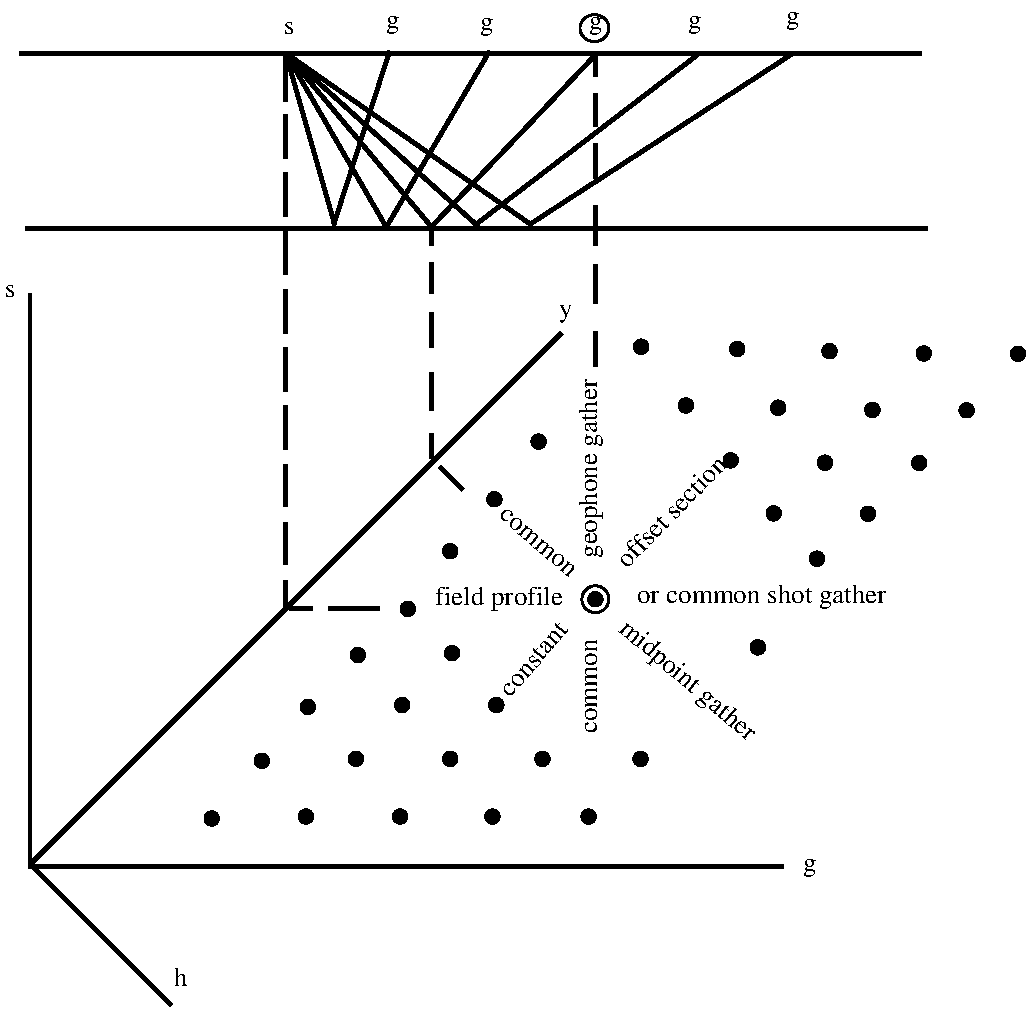
\includegraphics[width=0.65\textwidth]{ofs/sg}
\caption[sg]{顶部图为海上地震记录的野外记录排列,s为炮点,g为检波器。为有助于解释,图中有一水
平反射面。下面的图成为叠加图式(不是透视图)。平面上每个点表示一个可能的地震记录道,可以想象时间
轴是由该平面开始朝向平面之外的。顶部图中的中心检波器(带有圆圈标志者)记录了下图位置上(带圆圈者
)的地震记录道。下图中的各种标记给出了通用的显示名称}
\label{fig:ofs/sg}
\end{figure}

\begin{figure}[H]
\centering
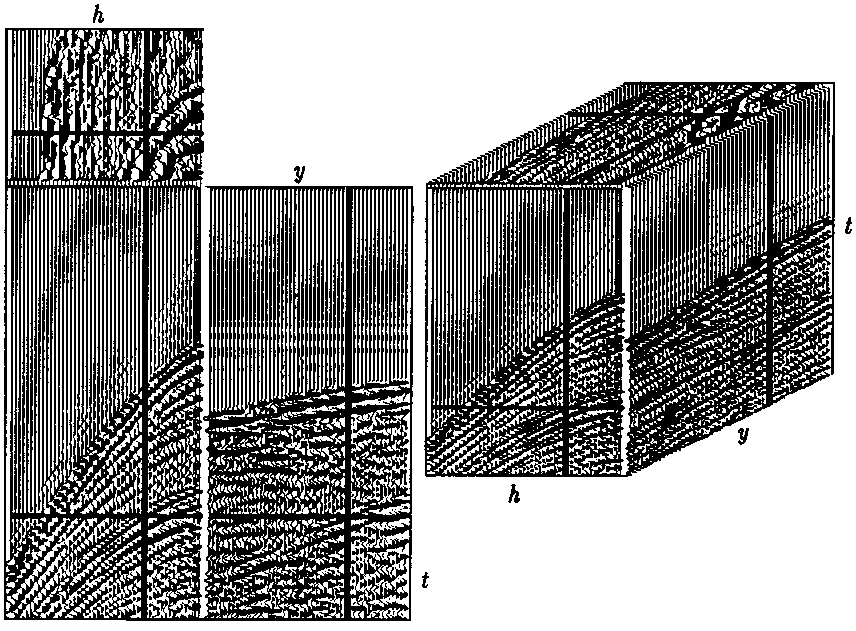
\includegraphics[width=0.65\textwidth]{ofs/rick}
\caption[rick]{Grand Bank地区的数据立方体之各个切片。左图为“工程画”模式,右图取自立方体内之
各切片均表示为立方体上的各侧面}
\label{fig:ofs/rick}
\end{figure}
共深度点(CDP)道集是由工业应用部门定义的,按惯例也可称为共中心点(CMP)
道集。但是在本书中,将对这二者加以区别:共深度点道集(CDP)将被认为是
时间坐标轴按某种速度模型业已拉伸了的共中心点道集(CMP)
\begin{equation*}
(y=const,h,\sqrt{t^2-4h^2/v^2} \quad commom-depth-point\quad gather
\end{equation*}
这种与炮检点有关的拉伸处理使得该道集的时间轴变得更像是深度轴,从而使CDP中的
D是真正与深度有关的。对时间轴进行的这种拉伸处理称作正常时差校正(NMO)。
注意,速度趋于无限大时,拉伸量就趋于零。

在实际应用中,并非按常规把数据显示成炮检距的函数,相反,每个CDP道集都遍及炮
检距求和,求和运算最终得出一个记录道。在每一中心点上可以构制出这样一个记录道,这
些记录道的集合是中心点和时间的函数,称作CDP叠加。粗略地说,CDP叠加剖面像是零
炮检距剖面,不过具有较少干扰的面貌罢了。

构制CDP叠加剖面要求对有利于时差校正的速度迸行选择,这样选择出的速度就称为叠
加速度。叠加速度可以只不过是对地层速度的某些猜涎,再不然用若干个试验速度进行叠
看一看哪个能得出能量最强而噪音最小的CDP叠加结果,因而使速度估计得到改善。在\ref{sec:3.5}
节内将对叠加处理作更多讨论。

图\ref{fig:ofs/profiles}为典型陆地剖面和海上
剖面(共炮点道集)。陆地资料系采用检波器位于震源两侧的方式记录,
所示该种野外布置称为不规则中间放炮排列,震源系人工连续震源。海上
资料碰巧能良好地显示有两个或三个
折射波(参阅\ref{sec:3.5}节与\ref{sec:5.2}节,海上震
源系采用汽枪。这些野外剖面每个均系采用120个左右的检波器所记录。
\begin{figure}[H]
\centering
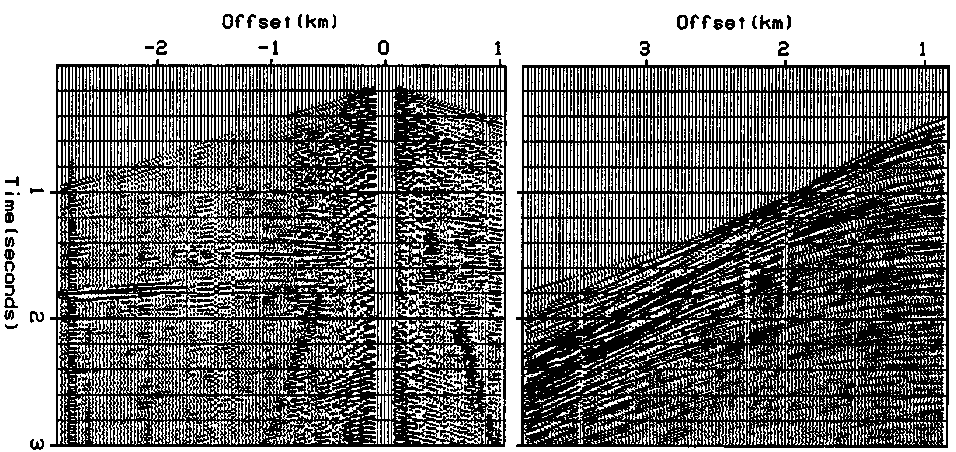
\includegraphics[width=0.65\textwidth]{ofs/profiles}
\caption[profiles]{野外剖面。左图为西得克萨斯的陆地剖面,右图为阿留申群岛附近的海上剖面}
\label{fig:ofs/profiles}
\end{figure}

\subsection{何谓“质量欠佳”资料?}
\label{sec:3.0.2}

世界广大地区有良好的石油储藏前景,但是由于获得质量良好的反射
地震资料很困难而难以勘探,其原因往往全都搞不清楚。到底何谓“质量
欠佳”资料?从野外工作的观点看,在记录均具有可重复性的意义下,几乎所有地震资料均可
算得上是良好的,现实问题却是该项资料可能毫无意义。

试取随机排列的点反射体作为地层模型,其经过偏移处理所得的零炮检距剖面看起来也
应是随机的。设数据采集是具有可重复性的,像这么一种具有随机面貌的资料只不过是暗示
有一堆杂乱随机的反射体而已。仅利用零炮检距资料,很少能再得出什么进一步的结论。但
是,在我们的处理中采用完整的炮检距范围时,则有可能进行更精细的分析。本章就是讨论
如此作时所需要的某些技术。

有一种有意义的地层模型,即点散射体在恒定速度介质内呈随机分布。所得数据将是时间
的随机函数和炮检距中点的水平位置之随机函数。但就每一中心点而言,该项数据在适当处
理之后却应完全是炮检距的一种双曲线形式的函数。这种双曲线能准确地确定逾层速度,即
使随机散射体呈三维分布而且仅沿地面测线进行记录时也是如此。

要想用这类特殊模型来解释“质量欠佳”资料,也可能是行不通的。在那种情形下,可
以试验一下采用其他一些模型。可以分析一下近地表处速度作随机变化所带来的影响或者分
析一下多次反射的影响,地震学中的噪音干扰通常可看作是分析失败的原因,而不看作是污
染了数据的某种什么东西。正是炮检距这个维数,给我们提供了为试图断定到底发生了什么
事情时所需要的冗余信息。

\subsection{水平分层结构、海上资料}
\label{sec:3.0.3}

重力是形成岩石成层现象的一种强大力量,在世界的许多地方,岩石均沉积为水平岩
层,即使在大多数理想沉积环境下,岩石层面也不是镜子般地光滑,它具有某种结抅特征。现
在我们用酷似非常理想的沉积环境的合成数据资料来开始我们的炮检距研究,这样一种环境
差不多肯定就是沉积作用能缓慢而又均勻地进行的海洋环境,波传播速度将取为常数,所有
射线将犹如是从水平伸展的镜面所反射的一般.从数学上说,允许岩层的反射系数横向可
变,就是弓丨入了岩层的结构特征,横向变化可假设成是一种随机函数,不过,没必要具有白
噪音谱。现在就让我们来研究一下如此形成的野外资料的面貌。

利用中心点$y$与深度$z$的一个随机函数将随机性质引入地层模型,这种随机性是沿深度$z$加
在某种连续迆质柱状剖面上的。对于$(y,z)$空间每一个点,必须在炮检距$h$与旅行时间$t$组
成的数据空间中沿着一个双曲线同相轴钯随机振幅叠加起来。

最终的数据空间是什么样子?在我们决定该三维数据体积究竟要怎样出现于眼前之前,
谈论这个问题是意义不大的。设我们把数据看成非常像在野外所记录到的那样,对于每个炮
点,我们看见一幅画面:其中的垂直轴是旅行时间而水平轴则是从船直到检波器拖缆的距离;
下一个炮点给我们另一个画面。如此重复,就使我们得到一部活动电影。这部电影所表现的
到底是什么呢?

单个画面表现的是具有给定结构特征的双曲线,活动电影表现的是沿每个双曲线向炮检
距増大方向移动着的结构特征(我发现没有一种静止图象的序列能给岀像活动电影给出的那
种印象)。实际上,船是真正在移动着,地层特征则稳定地位于其下。大多数海上资料的真正
样子就是这样,图\ref{lst:code3.0.4}所示计算机程序就是模拟它的。把合成数据同实际海上勘探资料相
比,我得到的印象是:要达到与野外资料相似,需要在合成资料内有大量随机横向变化。要
表示岩性变化,利用随机性似乎过分了一点,这显然是由于某些现象尚未能模拟所致。或许这
是由于我们对于从准随机性质的地层发生反射的机制还了解得不够完全的结果,或者也许它
就是波从次级不规则地形反射之后有时会出现局部聚焦所形成的影响。总之,完满的解释尚
有待于进一步研究。
\begin{listing}[H]
    \caption{模拟理想海上勘探条件下合成野外磁带的计算机程序}
    \inputminted{Fortran}{code-3-0.f90}
    \label{lst:code3.0.4}
\end{listing}

\subsection{陆地资料的特征:近地表影响问题}
\label{sec:3.0.4}

由于地表土壤层的不规则性,陆地记录的反射地震资料经常出现随机性。它往往如此之
糟以致地震震源必须深埋地下(费用很高),检波器因数量太多难以深埋。对于大多数陆地反
射资料而言,由这些表层不规则性所引起的特征超过了由反射层所形成的特征。

我们将提出一个理想的数学模型,以阐明我们的想法。设反射层平缓而无其他特征,检波
器均经受了若干时间采样点的随机时间延迟,这类时间延迟称为静校量。令震源具有随机的
强度。对这样形成的活动电影来说,设每个画面所表现的是在固定中心点$y$上的$(h,t)$空
间内之数据。就是说,设数据画面为共中心点道集;相继的画面所表现的将是相继的中心点
上的情况。对图\ref{fig:ofs/sg}迸行一番研究,你会确信:与检波器有关之旅行时间不规则性应朝左
移动,而与震源有关的振幅不规则性则应向右移动。在实际情形下,振幅异常与时间异常全都同
震源和检波器二者有关。

\subsection{习 题}
\label{sec:3.0.5}

\begin{enumerate}
\item 图\ref{fig:ofs/sg}是按炮点间隔$\Delta s$等于检波器间隔$\Delta g$的二分之一而绘制的。令
$\Delta s = \Delta g$,重新再绘制图\ref{fig:ofs/sg}。现在,有了两种类型的共中心点道集,试为
“近炮间距剖面”提出两种可能的定义。

\item 修改图\ref{lst:code3.0.4}所示程序,使它产生具有随机炮点振幅和随机检波
点时延的一种合成中心点道集活动电影。观察这种活动电影时你会注意
到,同向右的运动一起还能看到向左的运动,这是个感觉问题。试调节异常
强度使向左运动与向右运动模式二者全能看得清。
你心里总是想只看见一种运动,把另一种运动遮挡起来,这就类似于
你根据各个侧面的二维投影来感觉一个三维立方体一般。
\begin{figure}[H]
\centering
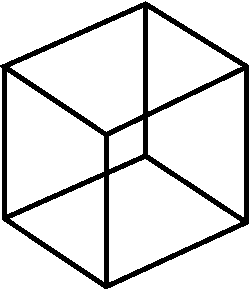
\includegraphics[width=0.5\textwidth]{ofs/cube}
\caption[cube]{立方体}
\label{fig:ofs/cube}
\end{figure}

\item 试设计出递妇倾角滤波器,使炮点、检波点及中心点的舞种不同特征能通过或截止。
\end{enumerate}
